
\chapter{Models for the artificial pancreas development}
\label{sec:ModelsForDiabetes}

% Se podria añadir un epigrafe con el quote de box "essentially, all models are wrong, but some are useful" http://en.wikiquote.org/wiki/George_E._P._Box

One of the main problems for glucose control is the insufficient accuracy of existing mathematical models for describing the physiology of the glucoregulatory system. In this chapter the modeling context for the artificial pancreas will be reviewed, and the state of the art of mathematical models in literature will be described.

\section{Introduction}
\label{sec:Introductionfodiabetes}

A mathematical model is characterized both by its objective and its structure. The main objective in modeling a type 1 diabetic subject is of course to be able to reproduce the patient's metabolism from a clinical point of view. In the artificial pancreas context, models must be useful from the control point of view. According to the structure of a model, quoting the work of Walter and Pronzato \cite{walter1997}, the main distinction to be made is whether a \textit{phenomenological} or \textit{behavioral} modeling approach must be followed. A phenomenological model is a model based on prior knowledge about physical or, in the case of the artificial pancreas, physiological principles. This kind of processes are often called \textit{knowledge-based} models as opposed to behavioral models, which merely approximate the observed behavior of the output without any prior knowledge of the process. Behavioral models are focused on data reproduction, and not at all in the process behind, while phenomenological models only use the data to adjust the parameters, while the structure is determined by the process itself.

Examples of phenomenological models are:
\begin{itemize}
	\item Chemical reactions. Biological reactions.
	\item Systems of force equilibrium.
	\item Models of deposit systems.
	\item Electromagnetic models. Electrical engines.
\end{itemize}
Examples of behavioral models are:
\begin{itemize}
	\item ARX/ARMAX models.
	\item Polynomial models.
	\item Random models.
\end{itemize}
The behavioral models exposed do not have the purpose of imitating any experimental process, and are ``all-purpose'' models that have to be adjusted to any particular system. On the contrary, the phenomenological models listed are specific of the process they represent. Table \ref{tab:PhenomenologicalAndBehavioralModels} shows a comparison of the differences between both modeling paradigms. In the context of the artificial pancreas almost every model published is phenomenological, even the simplest ones, due to the vast knowledge of the physiology available from the physicians. Behavioral models have also be used to characterize diabetic patients behavior, mostly in proof-of-concept studies like the ones performed by \cite{stahl2009diabetes}.
 
\begin{table}[hbtp]
	\centering
		\begin{tabular}{c|c|c}
		  &	Phenomenological models & Behavioral models \\
		 \hline 
		Parameters & have a concrete meaning & have no concrete meaning \\
		\hline 
		Simulation & long and difficult & quick and easy \\
		\hline 
		Prior information & taken into account & neglected \\
		\hline 
		Validity domain & large (if structure is correct) & restricted \\
		\end{tabular}
	\caption{Phenomenological and behavioral models as seen by Walter and Pronzato \cite{walter1997}.}
	\label{tab:PhenomenologicalAndBehavioralModels}
\end{table}

Usually, phenomenological models tend to be complex and highly nonlinear. Linearizing a phenomenological model changes its aim and its nature. When a nonlinear phenomenological model is designed, its aim is usually a better understanding of the system through simulation. Reasons for linearizing are usually attempts to control, or design of better controllers, but this transformation neglects the prior information of the system and its complexity, so the linearized model results in a behavioral model, with a restricted validity domain and lost of the experimental meaning of the parameters. A tradeoff between model complexity and accuracy is also imposed by the individualization of the model to an specific patient. Excessively complex models may struggle when fitting to an individual due to limitations of data available in the domiciliary context (data collected at home) yielding to lack of identifiability of the model. Loss of identifiability hinders parameter interpretation of the identified model, which is an important goal for physiology-based phenomenological models of diabetes.

Insulin treatment and meal ingestion can be posed as the input sub-models for the actual glucose endogenous regulation system. The outcome of the insulin infusion input model is the plasma insulin concentration, which is a main actor in glucose regulation, and works as an input to the endogenous system. Meal input works as a disturbance to the whole system, and the outcome of the related input system is the glucose flux into blood from the gut. In summary, physiological models of the glucose-insulin system for type 1 diabetes involve three main sub-processes:
\begin{itemize}
	\item \textbf{Insulin absorption model.} This model involves insulin pharmacokinetics, diffusion through different tissues and natural insulin degradation. Insulin absorption depends on the type of insulin used for the therapy and the route used for its delivery. Insulin is injected or infused in the subcutaneous tissue, delaying its appearance in plasma compared to insulin secretion by the pancreas. In case multiple daily injections are used, pharmacokinetics of both rapid-acting and long-acting insulin have to be considered. In case of insulin pumps (as in the artificial pancreas) only rapid-acting insulin is used.
	\item \textbf{Glucose absorption model.} Glucose input is represented in this model, which is also called the gastrointestinal model. It involves the process of ingestion, digestion and absorption from the intestine into blood of glucose and other nutrients. The nutritional composition of the meal influences the process of gastric emptying, affecting the flow of carbohydrates through the gut.
	\item \textbf{Glucoregulatory model.} The internal regulation of glucose is represented by this model. The transformation of glycogen to glucose by the liver (hepatic glucose production) and glucose uptake by peripheral tissues, the influence of different hormones in blood glucose, insulin independent consumption of glucose, and in summary, every effect that, in the organism, can affect the concentration in glucose. The models representing all these physiological processes and relations tend to be of high complexity, and it is really common to disregard some of the influences on the glucose concentration, so that the model becomes simpler and for other purposes than simulation.
\end{itemize}
The insulin absorption and gastrointestinal models are usually considered as the \textit{input models} for the glucose-insulin system, for they characterize the two main exogenous (coming from outside the body) inputs into blood that influence the glucose concentration (Figure \ref{fig:glucosemodels}). Several model reviews can be found in literature, being the most notorious Willinska's review \cite{wilinska2009simulation} and Nucci and Cobelli's review \cite{nucci2000models}, or the more recent one by Colmegna \textit{et al.} \cite{colmegna2014analysis}.

\begin{figure}[hbtp]
\centering
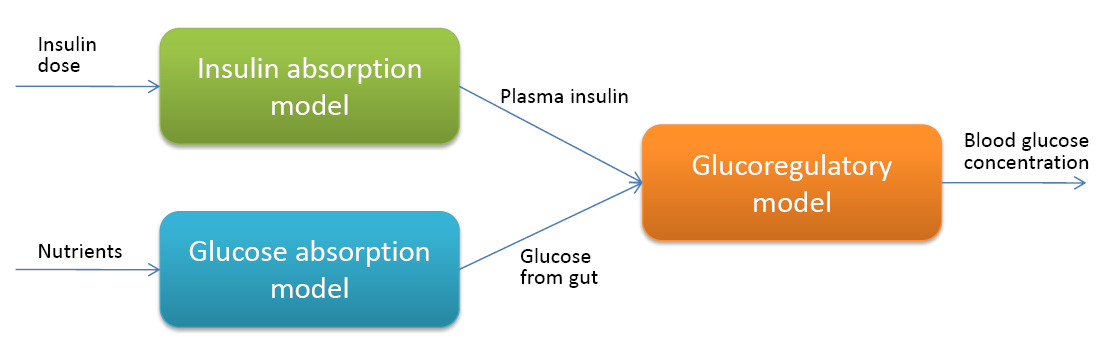
\epsfig{file=Figures/glucose_models.png, width=\textwidth}\caption{Glucose-insulin system and its sub-processes.}
\label{fig:glucosemodels}
\end{figure}

Subcutaneous insulin injection or pump delivery is the main control action to counteract disturbances like meal ingestion. Insulin pharmacokinetics has been studied for a long time, and the behavior of insulin analogues is well documented in literature. Complex glucose absorption models have been developed in the last years, but there still exist serious limitations to represent the physiological behavior of the digestive and intestinal absorption processes during a mixed meal mainly due to limitation of clinical data. The main difficulty in the characterization of the gastrointestinal model is that glucose absorption is only measurable with tracer methods \cite{basu2003use}, but few studies have been done in this area so far. The only experiments done in this area were not performed using real mixed meals, but instead the patients ate marked jelly with eggs and bacon. The influence of the nutritional composition is very relevant in the final model output, and it has not been taken in consideration so far.

Most commonly used models for the above mentioned systems will be introduced in the next sections, and later a critical review of the usefulness of these models will be performed in order to narrow down the scope of the research, not to forget that the last objective of this thesis is the identification of postprandial models for control.

\section{Insulin absorption models}
\label{sec:InsulinPharmacokineticsModels}

Modeling of subcutaneous (s.c.) insulin diffusion and absorption dates back to the 80's. Kobayashi \textit{et al.} published in 1983 a model based on a one-compartmental delay differential equation for U40 Actrapid insulin \cite{kobayashi1983pharmacokinetics} on type 1 and type 2 diabetic patients. Models proposed in literature have been increasing in complexity since then, like the two-compartmental model proposed by Kraegen \textit{et al.} in 1984 \cite{kraegen1984insulin}, or the model considering two different insulin pathways proposed by Puckett \textit{et al.} \cite{puckett1995model} in 1995. Increasing in complexity, Mosekilde \textit{et al.} proposed a model based on partial differential equations describing insulin dissociation, protein binding, diffusion and absorption \cite{Mosekilde1989modeling}. Later, Trajanoski \textit{et al.} simplified that model, and Tar\'in \textit{et al.} extended it's use to new insulin formulations, specifically to the insulin analog glargine \cite{tarin2005comprehensive}.

Works focused on the development of the artificial pancreas have studied in more detail the fast-acting insulin (e.g. lispro) used in insulin pumps. Wilinska \textit{et al.} from the University of Cambridge compared eleven different models for insulin lispro kinetics on data from seven patients with type 1 diabetes \cite{wilinska2005insulin}, concluding that the best performance was achieved by a model which considered two insulin absorption channels, a slow and a fast one. The group of Cambridge is one of the lead research teams for the artificial pancreas development, and they published a diabetic patient simulator in 2010 for \emph{in silico} testing of controllers \cite{simuladorhovorka}. However, a simplified version of the insulin absorption model was included, comprising a two-compartment single-path absorption structure, probably due to identifiability problems. The group of the University of Virginia and the University of Padova also published a simulator (henceforth UVA simulator) in 2007 \cite{magni2007model} with a very similar two compartment model. The models proposed by these two groups will now be displayed in more detail due to its widespread use.

\subsection{UVA model}
\label{sec:UVAins}

The model proposed by Dalla Man \textit{et al.} in 2007 \cite{man2007meal} has two compartments for the interstitial space and considers the elimination of insulin to happen entirely after the absorption to the plasma compartment. There are two variants of the model, depending on the complexity considered for the model of insulin distribution. The first and simpler model is the one shown in Figure \ref{fig:cobellisc1}. In this model, absorption takes place from both stages of the subcutaneous route.

\begin{figure}[hbtp]
\centering
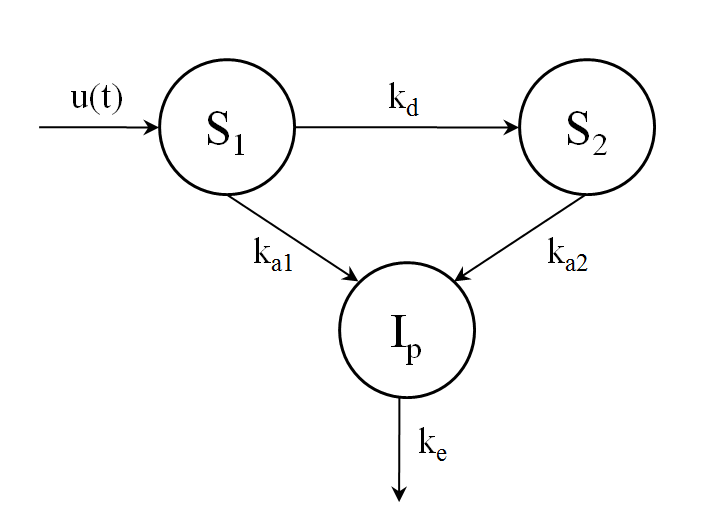
\epsfig{file=Figures/Cobelli1.png, width=0.6\textwidth}\caption{UVA model with one compartment for the insulin in plasma. Adapted from \cite{man2007meal}.}
\label{fig:cobellisc1}
\end{figure}

The equations related to the model are:
\begin{align}
	\dot{S}_{1}(t) &= -(k_{a1}+k_{d})S_{1}(t)+u(t) \label{eq:cobellisc1}\\
	\dot{S}_{2}(t) &= k_{d}S_{1}(t)-k_{a2}S_{2}(t) \label{eq:cobellisc2}\\
	\dot{I}_{p}(t) &= k_{a1}S_{1}(t)+k_{a2}S_{2}(t)-k_{e}I_{p}(t) \label{eq:cobellisc3}
\end{align}

where $S_{1}(t)$ and $S_{2}(t)$ are two compartments for the subcutaneous insulin absorption, $k_{a1}$, $k_{a2}$ and $k_{d}$ are the flux rates between compartments and plasma insulin ${I}_{p}(t)$, and $k_{e}$ is the insulin elimination rate. The insulin input is represented by the variable $u(t)$. Usually the subcutaneous part is used with a more complex insulin distribution and elimination model, also proposed by the Virginia and Padova group. The new model is displayed in Figure \ref{fig:cobellisc2}. In this case, elimination of insulin takes places both by degradation in the plasma compartment and in the liver. The influence of the liver is displayed by a new compartment.

\begin{figure}[hbtp]
\centering
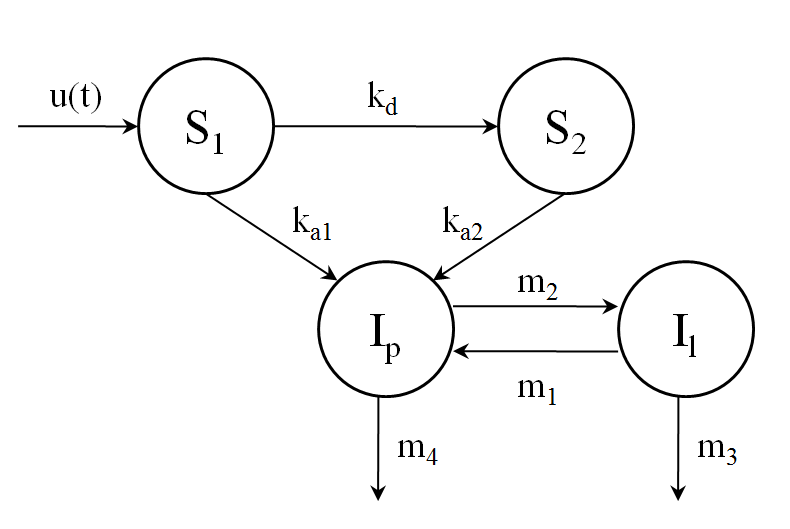
\epsfig{file=Figures/Cobelli2.png, width=0.6\textwidth}\caption{UVA model considering insulin in the liver and in plasma. Adapted from \cite{man2007meal}.}
\label{fig:cobellisc2}
\end{figure}

The corresponding system of equations related is very similar, but substituting equation \eqref{eq:cobellisc3}  with the following two differential equations:
\begin{align}
	\dot{I}_{l}(t) &= -(m_{1}+m_{3})I_{l}(t)+m_{2}I_{p}(t) \label{eq:cobellisc4}\\
	\dot{I}_{p}(t) &= -(m_{2}+m_{4})I_{p}(t)+m_{1}I_{l}(t)+ k_{a1}S_{1}(t)+k_{a2}S_{2}(t) \label{eq:cobellisc5}
\end{align}

where the plasma insulin elimination is replaced with a set of flux parameters ($m_1$, $m_2$, $m_3$ and $m_4$) and two dynamic states ($I_p$ and $I_l$) that represent insulin in plasma and the liver. Published values for T1DM patients were made available in 2008 in the international patent for the UVA simulator \cite{UVAsimpatente}. Public available values \cite{man2007meal} for healthy and T2DM patients for the distribution and elimination part of the model are shown in Table \ref{tab:cobelli_insulin}. Parameter $m_{3}$ does not appear in the table because it only is constant for T1DM patients while for the literature cases it presents dynamic behavior depending on the endogenous insulin secretion. Nevertheless, this model is implemented in the University of Virginia Simulator \cite{kovatchev2009biosimulation}, and nominal parameters for healthy and diabetic patients are used in glucose profiles simulated with it.

\begin{table}[hbtp]
	\centering
		\begin{tabular}{|c c c c|}
		\hline 
		Parameter &	Healthy value & T2DM value & Units \\
		\hline
		$m_{1}$ & $0.19$ & $0.379$ & min$^{-1}$ \\
		$m_{2}$ & $0.484$ & $0.673$ & min$^{-1}$ \\
		$m_{4}$ & $0.194$ & $0.269$ & min$^{-1}$ \\
		\hline		
		\end{tabular}
	\caption{Published values of the UVA s.c. insulin model.}
	\label{tab:cobelli_insulin}
\end{table}

\subsection{Cambridge model}
\label{sec:WillinskaEtAl}

In 2005 Willinska compared eleven subcutaneous models of increasing complexity \cite{wilinska2005insulin}. Those models where evaluated for bolus-basal treatments and continuous infusion with insulin pumps with insulin \textit{lispro}, a human insulin analog. The structure of the model with a better fit to experimental data is shown in Figure \ref{fig:willinska}.

\begin{figure}[hbtp]
\centering
\epsfig{file=Figures/Willinska.png, width=0.8\textwidth}\caption{Cambridge's model compartmental structure.Adapted from \cite{wilinska2005insulin}.}
\label{fig:willinska}
\end{figure}

The equations of the model are:
\begin{align}
	\dot{Q}_{1a}(t) &= ku(t)-k_{a1}Q_{1a}(t)-LD_{a}(t) \label{eq:Willinska1}\\
	\dot{Q}_{1b}(t) &= (1-k)u(t)-k_{a2}Q_{1b}(t)-LD_{b}(t) \label{eq:Willinska2}\\
	\dot{Q}_{2}(t) &= k_{a1}Q_{1a}(t)-k_{a1}Q_{2}(t)\label{eq:Willinska3}\\
	\dot{Q}_{3}(t) &= k_{a1}Q_{2}(t)+k_{a2}Q_{1b}(t)-k_{e}Q_{3}(t)\label{eq:Willinska4}\\
	I(t) &= \frac{Q_{3}(t)}{V_i\cdot BW} \label{eq:Willinska5}\\
	LD_{a}(t) &= \frac{V_{MAX,LD}Q_{1a}(t)}{k_{M,LD}+Q_{1a}(t)}\label{eq:Willinska6}\\
	LD_{b}(t) &= \frac{V_{MAX,LD}Q_{1b}(t)}{k_{M,LD}+Q_{1b}(t)}\label{eq:Willinska7}
\end{align}

The most significant characteristic of this model is the existence of two channels of insulin, one of slow absorption and a fast absorption insulin channel, both with degradation of insulin ruled by a Michaelis-Menten kinetic equation. ${Q}_{1a}(t)$ and ${Q}_{1b}(t)$ are the states related to slow insulin distribution in the subcutaneous tissue, ${Q}_{2}(t)$ is the state related to the fast distribution channel, and ${Q}_{3}(t)$ is directly related to the plasma insulin. $LD_{a}(t)$ and $LD_{ab}(t)$ describe insulin degradation with the constant parameters $V_{MAX,LD}$ and $k_{M,LD}$, $V_i$ is the insulin distribution volume, $BW$ is the patient's body weight and finally $k_{a1}$, $k_{a2}$ and $k_{e}$ are the constant fluxes and elimination rates between insulin compartments. The insulin concentration is directly calculated from the fourth compartment. Published parameters of the model are shown in Table \ref{tab:Willinska}.

\begin{table}[hbtp]
	\centering
		\begin{tabular}{|c c c|}
		\hline 
		Parameter &	Published value & Units \\
		\hline
		$k_{a1}$ & $1.12\cdot 10^{-2}$ & min$^{-1}$ \\
		$k_{a2}$ & $2.1\cdot 10^{-2}$ & min$^{-1}$ \\
		$k_{e}$ & $1.89\cdot 10^{-2}$ & min$^{-1}$ \\
		$k$ & $0.67$ & - \\
		$V_i$ & $56.45\cdot 10^{-2}$ & L kg$^{-1}$ \\
		$V_{MAX,LD}$ & $1.93$ & mU min$^{-1}$ \\
		$k_{M,LD}$ & $62.6$ & mU \\
		\hline		
		\end{tabular}
	\caption{Nominal values of the parameters in Willinska's model.}
	\label{tab:Willinska}
\end{table}

In the simulator published in 2010 \cite{simuladorhovorka} the Cambridge group implemented a much simpler linear compartmental model. The model structure is shown in Figure \ref{fig:willinska_simulator}.

\begin{figure}[hbtp]
\centering
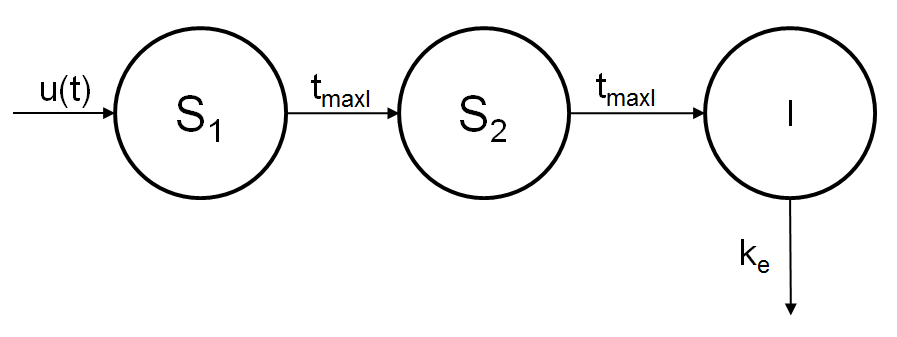
\epsfig{file=Figures/willinska_simulador.png, width=0.6\textwidth}\caption{Cambridge simulator insulin absorption model structure. Adapted from \cite{simuladorhovorka}.}
\label{fig:willinska_simulator}
\end{figure}

This model displays a simple flow of insulin through two compartments into the bloodstream, and it only considers elimination of insulin from blood. The flow constants between compartments is the same. The equations of this model are shown next:
\begin{align}
	\dot{S}_{1}(t) &= u(t)-t_{maxI}S_{1}(t) \label{eq:Willinska_simulator1}\\
	\dot{S}_{2}(t) &= t_{maxI}S_{1}(t)-t_{maxI}S_{2}(t) \label{eq:Willinska_simulator2}\\
	\dot{I}(t) &= \frac{t_{maxI}S_{2}(t)}{V_{i}}-k_{e}I(t)\label{eq:Willinska_simulator3}
\end{align}

The insulin compartment $I(t)$ is directly the insulin concentration. There are three parameters in this model: $t_{maxI}$ is the insulin absorption rate, $k_{e}$ is the elimination rate from the blood compartment, and $V_{i}$ is the insulin distribution. Willinska \textit{et al.} presented probability distributions of these parameters calculated from a population of 18 type 1 diabetic patients. For sake of simplicity and uniformity only mean values will be shown in this manuscript in Table \ref{tab:Willinska_simulador}, but the complete distributions can be found in \cite{simuladorhovorka}.

\begin{table}[hbtp]
	\centering
		\begin{tabular}{|c c c|}
		\hline 
		Parameter &	Published value & Units \\
		\hline
		$t_{maxI}$ & $0.018$ & min$^{-1}$ \\
		$k_{e}$ & $0.14$ & min$^{-1}$ \\
		$V_{i}$ & $0.12$ & L kg$^{-1}$ \\
		\hline		
		\end{tabular}
	\caption{Mean values of the parameters in the Cambridge simulator model.}
	\label{tab:Willinska_simulador}
\end{table}

\section{Glucose absorption models}	
\label{sec:GlucoseAbsorptionModels}

Glucose absorption models aim at characterizing the flux of exogenous glucose absorbed from the intestine under different circumstances taking under consideration the information on the meal intake. Modeling meal absorption has been proven difficult due to complex physiology of gastric emptying and intestinal absorption. The nature of the meal, its size and composition, as well as the speed of ingestion, and patient conditions, have influence on the rate of stomach emptying \cite{mitchell1989gastric} and the final absorption rate of glucose. Large variability was reported by Klingensmith \textit{et al.} \cite{klingensmith2010gastric} even within the same patient and meal. Furthermore, the rate of appearance of glucose in the bloodstream is not directly measurable (unlike blood insulin concentration in the insulin absorption models) which hardens the modeling endeavor.

One of the first models proposed in literature was an exponential model for gastric emptying presented in \cite{hunt1975volume}, where the emptying rate is dependent on the meal's volume and calorie density. After the contribution by Hunt \textit{et al.} most of the published models express the dynamics of glucose appearance as a function of the carbohydrate content of the meal. In 1992 Lehman and Deutch \cite{lehmann1992physiological} proposed a trapezoidal emptying of the stomach based on the carbohydrates ingested neglecting the influence of other nutrients. In 2006 Fabietti \textit{et al.} \cite{fabietti2006control} proposed an input-output model based on the different absorption rates of mono- and polysaccharides. A model independent approach was proposed by Herrero \textit{et al.} in \cite{bibliotecapau}, where the glucose absorption profile was extracted from a library comprehending several mixed meals and different patients. Also, deconvolution methods have been applied in order to infer the glucose absorption profile as proposed in \cite{herrero2012simple}.

In the simulators published up to date, physiological compartmental models are usually implemented. In the following lines we will describe in detail glucose absorption models from the UVA and Cambridge groups.

\subsection{UVA model}
\label{sec:ModelBasedOnDallaManEtAl}

Chiara Dalla Man \textit{et al.} published in 2006 a complete gastrointestinal model along with a critical review of the existing models in literature \cite{man2006system}. This model considers a two-compartment model for digestion and a simple single-compartmental model for the absorption in the gut. To overcome the issue of the measurability of glucose rate of appearance from the gut the UVA group used data from a triple tracer study, allowing for the estimation of glucose absorption, although in healthy subjects. The model follows the structure shown in Figure \ref{fig:dallaman}.

\begin{figure}[hbtp]
\centering
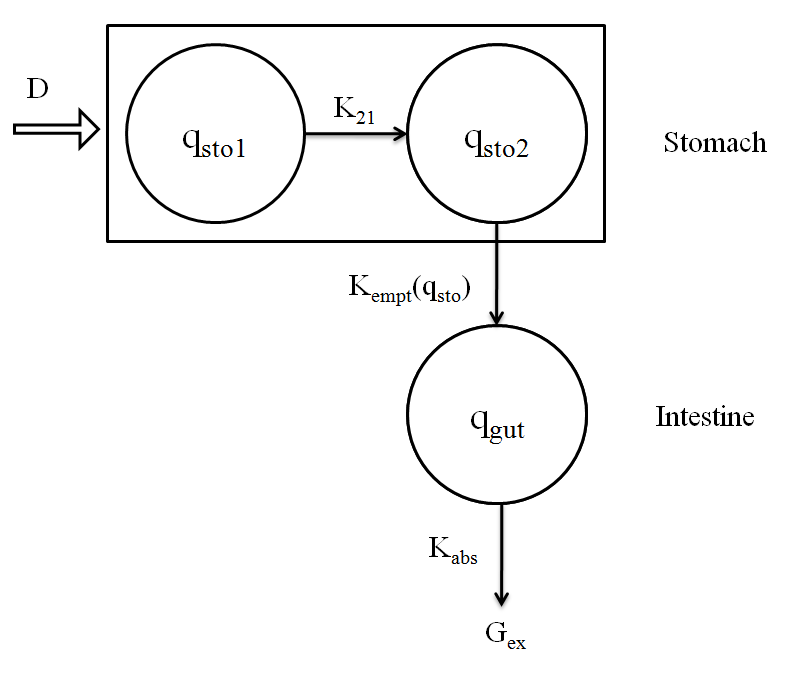
\epsfig{file=Figures/dallaman.png, width=0.6\textwidth}\caption{A two compartment model represents the stomach and a single compartment the intestine. Adapted from \cite{man2006system}.}
\label{fig:dallaman}
\end{figure}

The two compartments in the stomach part ($q_{sto1}$ and $q_{sto2}$) represent the solid and liquid phase of carbohydrate digestion before the gastric emptying. The emptying of the stomach is a non-linear function of the total amount of glucose in the stomach, as will be shown in the model equations later. The compartmental model equations are:
\begin{align}
  \dot{q}_{sto1}(t) &=-K_{21}q_{sto1}(t)+D\delta (t)\label{eq:dallaman1}\\
  \dot{q}_{sto2}(t) &=-K_{empt}(q_{sto})q_{sto2}(t)+K_{21}q_{sto1}(t)\label{eq:dallaman2}\\
  \dot{q}_{gut}(t) &=-K_{abs}q_{gut}(t)+K_{empt}(q_{sto})q_{sto2}(t)\label{eq:dallaman3}\\
  G_{ex}(t) &=fK_{abs}q_{gut}(t)\label{eq:dallaman4}
\end{align}
where $\delta (t)$ is the Dirac delta and $D$ is the meal size, simulating an impulse input to the model. $f$ stands for the bio-availability of the meal. The rest of parameters added ($K_{21}$ and $K_{abs}$) are flux constants between compartments, for characterization of the transfer of glucose through the system, except for the $K_{empt}$ parameter, which is time-varying and defines the form of the gastric emptying. The equations describing the transfer rate describing the flow of glucose from the stomach to the intestine are:
\begin{equation} \label{eq:dallaman5}
\begin{array}{ll}
  K_{empt}(q_{sto}) &= K_{min}+\frac{K_{max}-K_{min}}{2}\cdot\\
  & \hskip -1.5cm \cdot \{ tanh[\alpha (q_{sto}(t)-b\cdot D)]-tanh[\beta (q_{sto}(t)-c\cdot D)]+2\}\\
\end{array}
\end{equation}
\begin{equation} \label{eq:dallaman6}
  q_{sto}(t) =q_{sto1}(t)+q_{sto2}(t)\\
\end{equation}
\begin{equation} \label{eq:dallaman7}
  \alpha = \frac{5}{2D(1-b)}; \qquad   \beta = \frac{5}{2Dc} \\
\end{equation}
These equations give the gastric emptying a very characteristic shape. In Figure \ref{fig:dallaman2} the $K_{empt}$ is plotted against the amount of glucose remaining in the stomach $q_{sto}$.

\begin{figure}[hbtp]
\centering
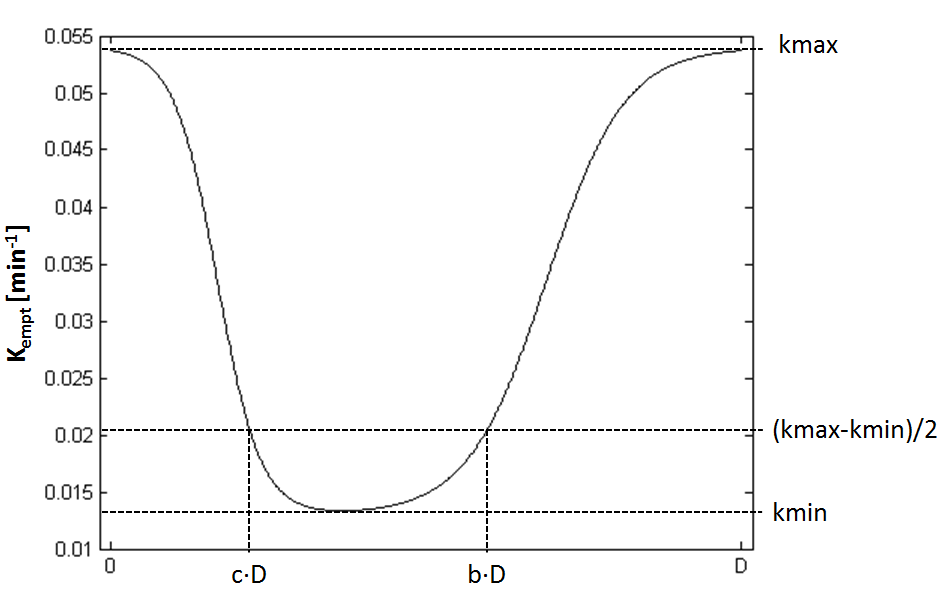
\epsfig{file=Figures/dallaman2.png, width=0.8\textwidth}\caption{Gastric emptying rate versus glucose remaining in the stomach. Adapted from \cite{man2006system}.}
\label{fig:dallaman2}
\end{figure}

$K_{max}$ and $K_{min}$ are the maximum and minimum emptying rates through the digestion process, while $b$ and $c$ are geometric parameters describing the shape of the gastric emptying. The parameters shown next have been identified both for an Oral Glucose Tolerance Test (OGTT, consisting in 75g of oral glucose ingestion according to the World Health Organization recommendation) and a mixed meal, although the mixed meal consisted only of traced jelly with eggs and bacon. Parameter $K_{21}$ is forced to be equal to $K_{max}$ for identifiability issues. The published values are shown in Table \ref{tab:dallaman}.

\begin{table}[hbtp]
	\centering
		\begin{tabular}{|c c c c|}
		\hline 
		Parameter & Published value (OGTT) & Published value (meal) & Units \\
		\hline 
		$K_{abs}$ & $0.205$ & $0.071$ & min$^{-1}$ \\
		$K_{21}$ & $0.045$ & $0.054$ & min$^{-1}$ \\
		$K_{max}$ & $0.045$ & $0.054$ & min$^{-1}$ \\
		$K_{min}$ & $0.013$ & $0.006$ & min$^{-1}$ \\
		$b$ & $0.85$ & $0.69$ & - \\
		$c$ & $0.25$ & $0.17$ & - \\
		\hline
		\end{tabular}
	\caption{Nominal values of the parameters in the UVA model.}
	\label{tab:dallaman}
\end{table}

%Some work has been done within this research group on identifiability of mixed meals with the Dalla Man model \cite{tesinacrisos}, showing a dependence of the identification results on the size of the meal considered.

\subsection{Cambridge model}
\label{sec:ModelBasedOnHovorkaEtAl}

Hovorka \textit{et al.} proposed a simple model for glucose absorption in 2004 \cite{hovorka2004nonlinear}, where the gastrointestinal system is modeled by two identical compartments with the same transfer rate. Later, the model was refined \cite{simuladorhovorka} considering the transfer rate $t_{max}$ as a time-varying parameter. The equations of the model are:
\begin{align}
	\dot{G}_{1}(t) &=-\frac{G_{1}(t)}{t_{max}}+Bio\cdot D(t) \label{eq:hovorkagut1}\\
	\dot{G}_{2}(t) &=\frac{G_{1}(t)}{t_{max}}-\frac{G_{2}(t)}{t_{max}} \label{eq:hovorkagut2}\\
	G_{ex}(t) &=\frac{G_{2}(t)}{t_{max}} \label{eq:hovorkagut3}
\end{align}
where:
\begin{itemize}
	\item \textbf{$D(t)$} is the amount of carbohydrates ingested in grams. The meal intake in this model is considered as a pulse input.
	\item \textbf{$Bio$} is the effectiveness of the absorption of the carbohydrates ingested, i.e. the portion of the carbohydrates that have been eaten that will go into the circulatory system (Bioavailability).
	\item \textbf{$t_{max}$} is the maximum absorption time of the carbohydrates. This parameter regulates the transfer speed between the compartments. It is a bounded parameter following:
	\begin{equation} 
	  t_{max}=\left\{ \begin{array}{cc} 
	  t_{max\ ceil} & \mbox{ if } G_{ex} > G_{ex\ ceil} \\ 
	  t_{max} & \mbox{ otherwise } \\	
	  \end{array} \right.
	\label{eq:hovorkagut4}
	\end{equation}
	where $t_{max\ ceil}=\frac{G_{2}}{G_{ex\ ceil}}$ and $G_{ex\ ceil}$ is the maximum glucose flux from the gut.
	\item \textbf{$G_{ex}(t)$} is the output of the model, as a flux of glucose from the gut. $G_{1}(t)$ and $G_{2}(t)$ are the transition compartments for glucose in the disgestion process.
\end{itemize}
The nominal values of the parameters are shown in Table \ref{tab:hovorkagut}.

\begin{table}[hbtp]
	\centering
		\begin{tabular}{|c c c|}
		\hline 
		Parameter & Published value & Units \\
		\hline 
		$t_{max}$ & $40$ & min \\
		$Bio$ & $0.8$ & - \\
		$G_{ex\ ceil}$ & $[0.02, 0.035]$ & mmol kg$^{-1}$ min$^{-1}$ \\
		\hline
		\end{tabular}
	\caption{Nominal values of the parameters in Hovorka model.}
	\label{tab:hovorkagut}
\end{table}

This model has the weakness of not considering the different compositions of mixed meals, as other models do, but it computes a very simple input for the glucoregulatory system in the simulation environment.

\section{Endogenous models}
\label{sec:EndogenousModels}

The endogenous model is the part of the glucose-insulin model that describes the different regulatory metabolic pathways of blood glucose concentration. Given that this thesis is focusing in the identification of glucose metabolism for T1DM subjects, the author decided that the dynamics and equations describing the secretion of insulin were no relevant to be shown for those models that describe it, since it does not exist in type 1 diabetes.

Usually the endogenous model comprises two sub-models: (1) insulin pharmacodynamics and (2) glucose metabolism and distribution. This second sub-model has to consider the influence of the liver and the kidneys on the blood glucose production and elimination, as well as the peripheral intake by muscles and adipose tissue, and any other influences that may affect glucose concentration. 

Two different groups of models will be described next. The first two models (Bergman and Panunzi) are considered as \textit{minimal} models, and are very simple models that do not attempt at simulating the whole metabolic system of glucose regulation but to capture the main dynamics in specific assays like the Intra Venous Glucose Tolerance Test (IVGTT) for insulin sensitivity estimation. Minimal models are widely used for research either in simulation studies or for control, but lack the accuracy of more complex models. The other two models reviewed next are physiology-based models developed by the UVA group and the Cambridge group, and are much more complex than the previous ones, aiming at population studies for controllers validation.

\subsection{Bergman model}
\label{sec:BergmanEtAl}

The first model to be reviewed is the (probably) most used and best known among all the endogenous models used in diabetes. It was proposed by Bergman \textit{et al.} in 1981 \cite{bergman1981physiologic}. It is considered a minimal model because it only describes the influence of insulin on blood glucose concentration, and it does not consider many other phenomena, or it considers them in a very simplified way, leading to a low order model. The justification for this simplicity is that the objective of this model was, initially, to simulate the response of the IVGTT, which has a very simple behavior.

Bergman minimal model considers that insulin actions on glucose are delayed, and that delay is represented by a new compartment of \textit{remote} insulin. The scheme of the model is shown in Figure \ref{fig:bergman1}.

\begin{figure}[hbtp]
\centering
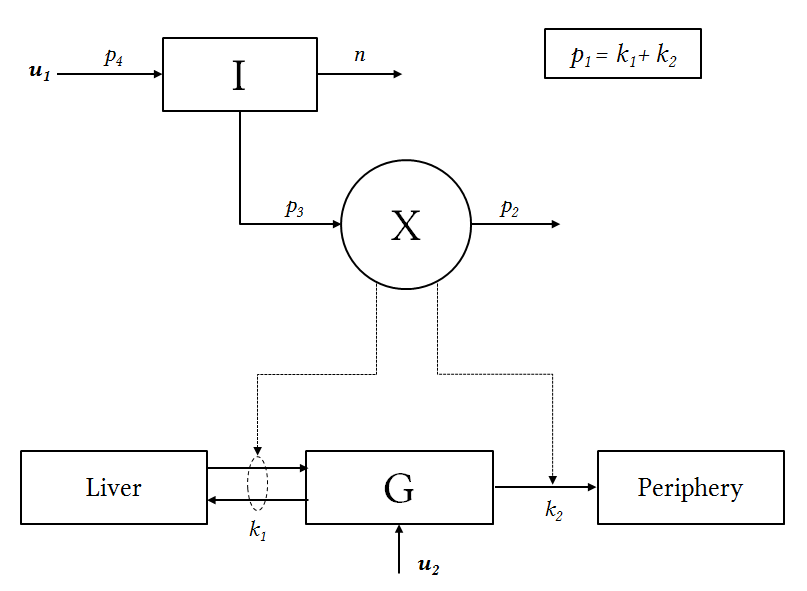
\epsfig{file=Figures/bergman.png, width=0.8\textwidth}\caption{Bergman minimal model of insulin and glucose dynamics. Adapted from Bergman and colleagues \cite{bergman1981physiologic}.}
\label{fig:bergman1}
\end{figure}

The equations that describe the model are:
\begin{align}
  \dot{I}(t) &= -nI(t)+p_{4}u_{1}(t) & I(0)=I_{b}=\frac{p_{4}}{n}u_{1b} \label{eq:Bergman1}\\
  \dot{X}(t) &= -p_{2}X(t)+p_{3}[I(t)-I_{b}] & X(0)=0 \label{eq:Bergman2}\\
  \dot{G}(t) &= -p_{1}G(t)-X(t)G(t)+p_{1}G_{b} + \frac{u_{2}(t)}{V_{G}} & G(0)=G_{b} \label{eq:Bergman3}
\end{align}

where the insulin compartment is described by the state $I(t)$, with parameters $p_4$ and $n$ involved in the insulin input and elimination respectively. Parameters $p_3$ and $p_2$ describe the input and output fluxes for the remote insulin compartment $X(t)$, and finally glucose difusion and transportation is gobernated by parameter $p_1$, which is a compound parameter involving both liver interaction ($k_1$) and usage by periphery ($k_2$). For subcutaneous insulin absorption, equation \eqref{eq:Bergman1} would be substituted by the corresponding model in Section \ref{sec:InsulinPharmacokineticsModels}. $G(t)$ is the blood glucose concentration, $u_{1}(t)$ is the exogenous insulin flow entering circulation, $u_{2}(t)$ is the exogenous flow of glucose coming either intravenously or from the gastrointestinal system. Published values for the model parameters are shown in Table \ref{tab:Bergman}.

\begin{table}[hbtp]
	\centering
	\begin{tabular}{|c c c|}
	\hline 
	Parameter & Published value & Units \\
	\hline 
	$p_{1}$ & $0.035$ & min$^{-1}$ \\
	$p_{2}$ & $0.05$ & min$^{-1}$ \\
	$p_{3}$ & $0.000028$ & ml$/\mu U\cdot$ min$^{2}$ \\
	$p_{4}$ & $0.098$ & ml$^{-1}$ \\
	$n$ & $0.142$ & min$^{-1}$ \\
	$V_{G}$ & $117$ & dl\\
	\hline
	\end{tabular}
\caption{Nominal values of the parameters in Bergman model \cite{roy2007dynamic}.}
\label{tab:Bergman}
\end{table}

Bergman model has been used for more than 20 years in diabetes research due to its identifiability and controllability properties, despite its simplicity. Nevertheless, Bergman model will be analyzed in detail in Section \ref{sec:BergmanEtAl}.

\subsection{Panunzi model}
\label{sec:PanunziEtAl}

Simona Panunzi \textit{et al.} published a study in 2007 comparing some of the characteristics of Bergman model and new features of a proposed model for the IVGTT scenario, with a delayed insulin secretion rate \cite{panunzi2007discrete}. The new model proposed surpassed the rest in simulated experiments and in identifiability properties, but it was only tested in healthy patients. The equations of the model are:
\begin{align}
  \dot{G}(t) &= -K_{xgl}I(t)G(t) +\frac{T_{gh}}{V_{g}} \label{eq:Panunzi1} \\
  \dot{I}(t) &= -K_{xi}I(t)+\frac{T_{ig\ max}}{V_{i}}\frac{\left(\frac{G(t-\tau_{g})}{G^{*}}\right)^{\gamma}}{1+\left(\frac{G(t-\tau_{g})}{G^{*}}\right)^{\gamma}} \label{eq:Panunzi2}
\end{align}
This model includes delayed differential equations for the insulin production sub-model, but when simulating type 1 diabetic patients, whom do not have endogenous insulin secretion, the model becomes much more simple. The parameters involved in the previous model are:
\begin{itemize}
	\item \textbf{$G_{b}$} is the basal glucose concentration.
	\item \textbf{$I_{b}$} is the basal plasma insulin.
	\item \textbf{$K_{xgl}$} is the insulin sensitivity. It represents the insulin-dependent glucose uptake by tissues per unit of insulin concentration.
	\item \textbf{$T_{gh}$} represents the balance between the hepatic glucose production of glucose and the insulin-independent glucose intake, including the one of the liver.
	\item \textbf{$V_{g}$} is the apparent glucose distribution volume.
	\item \textbf{$K_{xi}$} is the disappearance rate of insulin.
	\item \textbf{$G^{*}$} is the glycemia at which the insulin secretion rate is half of its maximum.
	\item \textbf{$T_{ig\ max}$} is the maximum rate of insulin release.
	\item \textbf{$V_{i}$} is the apparent insulin distribution volume.
	\item \textbf{$\tau_{g}$} represents the apparent delay with which the pancreas changes insulin release in response to a variation in blood glucose.
	\item \textbf{$\gamma$} is the progressivity with which the pancreas reacts to circulating glucose concentrations.
\end{itemize}
The values published for these parameters, only for healthy patients, are shown in Table \ref{tab:panunzi}.

\begin{table}[hbtp]
	\centering
		\begin{tabular}{|c c c|}
		\hline 
		Parameter & Published value & Units \\
		\hline 
		$V_{g}$ & $0.152$ & L\ kg$^{-1}$ \\
		$\tau_{g}$ & $19.271$ & min \\
		$K_{xgl}$ & $1.43\times 10^{-4}$ & min$^{-1}$ \ pM$^{-1}$ \\
		$K_{xi}$ & $0.101$ & min$^{-1}$ \\
		$\gamma$ & $2.464$ & - \\
		\hline
		\end{tabular}
	\caption{Nominal values of the parameters in Panunzi model.}
	\label{tab:panunzi}
\end{table}

Panunzi model is also used later in this thesis because of its simplicity, but some variations were made in Chapter \ref{sec:CriticalSelectionOfModels} due to the focus of this model on healthy patients and the IVGTT scenario, and in order to extend its use to diabetic patients.

\subsection{UVA model}
\label{sec:CobelliEtAl}

The core of the UVA model was presented in \cite{man2007meal}, and it is one of the most important models in diabetes research. It is a very complex model almost exclusively based on physiological knowledge of the glucose metabolism. It is usually combined with the UVA gastrointestinal model and the insulin pharmacokinetics model of the same group (in fact all the models were developed together) in a large mathematical model of the glucose metabolism. Magni \textit{et al.} \cite{magni2007model} used a linearization of the UVA model to control an \textit{in silico} diabetic patient. It is also the model implemented in the UVA simulator \cite{kovatchev2009biosimulation} which was accepted by the FDA (Food \& Drug Administration) as substitute of animal trials in the context of a controller validation trial by University of Virginia and Padova. The core structure is pretty simple, as shown in Figure \ref{fig:cobelliendo}:

\begin{figure}[hbtp]
\centering
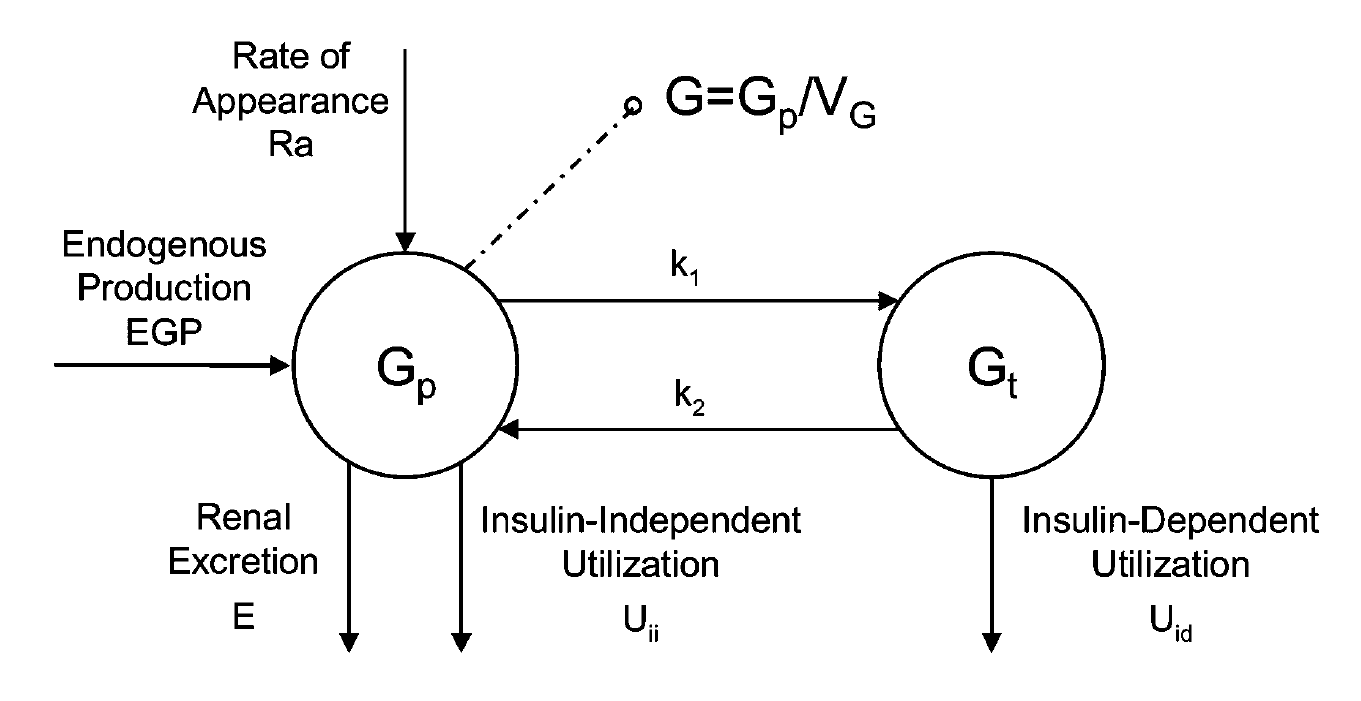
\epsfig{file=Figures/cobelliendo.png, width=0.8\textwidth}\caption{UVA's model core is composed of two compartments of glucose, one for blood and one for the tissues interstitial fluid. Schematics adapted from \cite{man2007meal}}
\label{fig:cobelliendo}
\end{figure}

The model equations are:
\begin{align}
  \dot{G}_{p}(t) &= EGP(t) + Ra(t) - U_{ii}(t) - E(t) - k_{1}G_{p}(t) + k_{2}G_{t}(t) \label{eq:cobelli1} \\
  \dot{G}_{t}(t) &= -U_{id}(t) + k_{1}G_{p}(t) - k_{2}G_{t}(t) \label{eq:cobelli2} \\
  G(t) &=G_{p}(t)/V_{G} \label{eq:cobelli3}
\end{align}
In the previous equations there are many inputs and outputs to the glucose compartments that need description. It must be noted that so far there are no insulin related equations; insulin influences the flow of glucose coming in or out of the different compartments. The meaning of these variables is explained next:
\begin{itemize}
	\item $Ra$ is the exogenous flux of glucose coming from the gut.
	\item $U_{ii}$ is the utilization of glucose that is non dependent on insulin. It is usually considered constant and equal to $F_{cns}$. 
	\item $U_{id}$ is the utilization that depends on the insulin concentration, and it follows the following set of equations:
  \begin{align}
  	\dot{X}(t) &= -p_{2U}X(t)+p_{2U}[I(t)-I_{b}]\label{eq:cobelli4} \\
  	V_{m}(X(t)) &= V_{m0}+V_{mx}X(t) \label{eq:cobelli5} \\
		U_{id}(t) &= \frac{V_{m}(X(t))G_{t}(t)}{K_{m}+G_{t}(t)} \label{eq:cobelli6}
	\end{align}	
	where $X(t)$ is the remote insulin, $I(t)$ is the plasma insulin, $I_{b}$ is the basal insulin and $V_{m}(t)$ is the transfer rate for the Michaelis-Menten equation shown in equation \eqref{eq:cobelli6}.
  \item $E(t)$ represents the renal excretion, which occurs if plasma glucose exceeds a certain threshold. It is modeled as follows:
  \begin{equation}
	E(t) = \left\{
		\begin{array}{cc} k_{e1}[G_{p}(t)-k_{e2}] & \mbox{ if } G_{p}(t)>k_{e2} \\
		0 &\mbox{ otherwise } 
		\end{array} \right.
  \label{eq:cobelli7}
  \end{equation}
  where $k_{e1}$ is the glomerular filtration rate and $k_{e2}$ is the renal threshold of glucose.
  \item $EGP(t)$ is the Endogenous Glucose Production, and it depends on a delayed insulin signal as follows:
  \begin{align}
  	\dot{I}_{1}(t) &= -k_{i}[I_{1}(t)-I(t)] \label{eq:cobelli8} \\
  	\dot{I}_{d}(t) &= -k_{i}[I_{d}(t)-I_{1}(t)] \label{eq:cobelli9} \\
		EGP(t) &= max\{0,k_{p1}-k_{p2}G_{p}(t)-k_{p3}I_{d}(t)\} \label{eq:cobelli10}
	\end{align}
	where $I(t)$ is the insulin concentration in plasma, $I_d(t)$ is the delayed insulin action, $k_i$ is the insulin delay flux rate and $k_{p1}$, $k_{p2}$ and $k_{p3}$ are constant parameters that describe $EGP$.
\end{itemize}
The published parameters for healthy and type 2 diabetic patients are those in Table \ref{tab:cobelli}. %Even though the parameters shown are those of healthy and T2DM patients, no endogenous production of glucose has been described in here for this model, which is the case of a T1DM person. 
\begin{table}[hbtp]
	\centering
		\begin{tabular}{|c c c c|}
		\hline 
		Parameter & Healthy & Type 2 diabetes & Units \\
		\hline 
		$V_{G}$ & $1.88$ & $1.49$ & dL\ kg$^{-1}$ \\
		$k_{1}$ & $0.065$ & $0.042$ & min$^{-1}$ \\
		$k_{2}$ & $0.079$ & $0.071$ & min$^{-1}$ \\
		$k_{p1}$ & $2.70$ & $3.09$ & mg\ kg$^{-1}$\ min$^{-1}$ \\
		$k_{p2}$ & $0.0021$ & $0.0007$ & min$^{-1}$ \\
		$k_{p3}$ & $0.009$ & $0.005$ &  mg\ kg$^{-1}$\ min$^{-1}$ per pmol L$^{-1}$ \\
		%$k_{p4}$ & $0.0618$ & $0.0786$ & mg\ kg$^{-1}$\ min$^{-1}$ per pmol kg$^{-1}$ \\
		$k_{i}$ & $0.0079$ & $0.0066$ & min$^{-1}$ \\
		$F_{cns}$ & $1$ & $1$ &  mg\ kg$^{-1}$\ min$^{-1}$ \\
		$V_{m0}$ & $2.5$ & $4.65$ &  mg\ kg$^{-1}$\ min$^{-1}$ \\
		$V_{mx}$ & $0.047$ & $0.034$ &  mg\ kg$^{-1}$\ min$^{-1}$ per pmol L$^{-1}$ \\
		$K_{m0}$ & $225.59$ & $466.21$ & mg\ kg$^{-1}$ \\
		$p_{2U}$ & $0.0331$ & $0.0840$ & min$^{-1}$ \\
		$k_{e1}$ & $0.0005$ & $0.0007$ & min$^{-1}$ \\
		$k_{e2}$ & $339$ & $269$ & mg\ kg$^{-1}$ \\
		\hline
		\end{tabular}
	\caption{Nominal values of the parameters in Cobelli model.}
	\label{tab:cobelli}
\end{table}

This model has been used in several experimental settings for closed-loop controller testing. Kovatchev \textit{et al.} published a study on 20 T1DM patients using an MPC controller tuned with the UVA simulator \cite{kovatchev2010multinational} \cite{clarke2009closed}. Improvement was reported in hypoglycemic events occurrence and in the amount of time spent in euglycemic range. Currently, the UVA group is performing home control experiments using controllers designed with this model.

An update of the UVA model and its simulator was published in January 2014 \cite{dalla2014uva}. The model is still based on the previous equations, but glucagon kinetics are included using a single compartment model. In order to simulate different glucose utilization depending on the glycemic region, the updated model includes a new glucose utilization module that depends on the risk of hypoglycemia. These last updates were not subject to examination in this thesis.

\subsection{Cambridge model}
\label{sec:HovorkaEtAl}

The Cambridge group proposed an endogenous model with split focus on three insulin actions and its final effect on blood glucose \cite{hovorka2002partitioning}. The model considers the following insulin effects:
\begin{itemize}
  \item Insulin increases the flow of glucose from blood to the tissues.
  \item Insulin increases the glucose uptake by muscles and adipose tissue.
  \item Insulin inhibits production of glucose in the liver.
\end{itemize}
These three influences are reflected in the model as virtual compartments. The relation between actual insulin in plasma, every virtual compartment representing insulin actions and the two compartments for glucose is shown in Figure \ref{fig:hovorka}. $x_{1}$, $x_{2}$ and $x_{3}$ represent the insulin actions, $Q_{1}$ is the glucose mass in the accessible compartment, and $Q_{2}$ is the glucose present in the non-accessible compartment. 

\begin{figure}[hbtp]
\centering
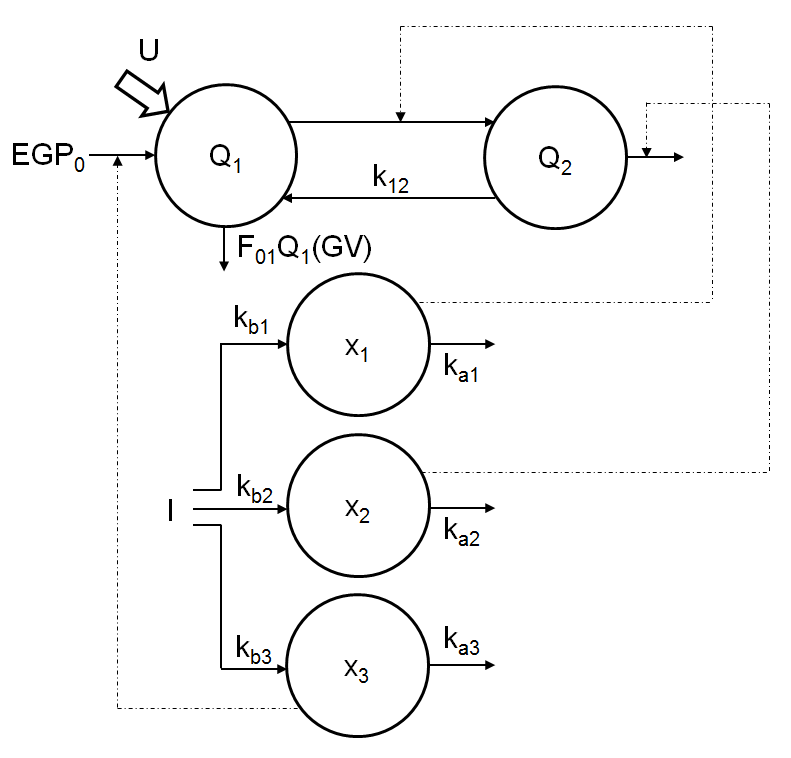
\epsfig{file=Figures/hovorka.png, width=0.8\textwidth}\caption{Hovorka endogenous model structure arranged in compartments. Adapted from \cite{hovorka2002partitioning}.}
\label{fig:hovorka}
\end{figure}

The equations that represent this model are:
\begin{align}
  \dot{x}_{1}(t) &= -k_{a1}x_{1}(t) + k_{b1}I(t) &  x_{1}(0)=0 \label{eq:hovorka1} \\
  \dot{x}_{2}(t) &= -k_{a2}x_{2}(t) + k_{b2}I(t) &  x_{2}(0)=0 \label{eq:hovorka2} \\
  \dot{x}_{3}(t) &= -k_{a3}x_{3}(t) + k_{b3}I(t) &  x_{3}(0)=0 \label{eq:hovorka3}
\end{align}

where $x_1(t)$, $x_2(t)$ and $x_3(t)$ are the three different insulin actions. These actions are used as inputs to the actual endogenous model.
%\begin{align}
%	\dot{Q}_{1}(t) &= -\left[\frac{F_{01}^{c}(t)}{V_{G}G(t)}+x_{1}(t)\right]Q_{1}(t)+k_{12}Q_{2}(t)-&F_{R}(t)+EGP(t)+&G_{ex}(t) \nonumber \\ 
%	& & Q_{1}(0)=Q_{1,0}& \label{eq:hovorka4} \\
%  \dot{Q}_{2}(t) &= x_{1}(t)Q_{1}(t)-[k_{12}+x_{2}(t)]Q_{2}(t) &Q_{2}(0)=Q_{2,0}& \label{eq:hovorka5} \\
%  G(t) &= Q_{1}(t)/V_{G} & &\label{eq:hovorka6}
%\end{align}
\begin{align} 
\begin{split} \label{eq:hovorka4}	\dot{Q}_{1}(t)= & -\left[\frac{F_{01}^{c}(t)}{V_{G}G(t)}+x_{1}(t)\right]Q_{1}(t)+k_{12}Q_{2}(t)- \\	& -F_{R}(t)+EGP(t)+G_{ex}(t) \quad \quad \quad \, Q_{1}(0)=Q_{1,0} \end{split} \\
  \dot{Q}_{2}(t)= & x_{1}(t)Q_{1}(t)-[k_{12}+x_{2}(t)]Q_{2}(t) \quad \quad \, Q_{2}(0)=Q_{2,0} \label{eq:hovorka5} \\
  G(t)= & Q_{1}(t)/V_{G} \label{eq:hovorka6}
	\end{align}

Equation \eqref{eq:hovorka4} has several terms to be defined:
\begin{itemize}
  \item $Q_1(t)$ is the compartment of plasma glucose.
	\item $Q_2(t)$ is the compartment of glucose in the interstitium.
	\item $G_{ex}(t)$ is exogenous flow os glucose.
	\item \textbf{$EGP$} stands for Endogenous Glucose Production, which is the flux of glucose coming from the liver. It is defined as:
	\begin{equation}
		EGP(t) = \left\{
			\begin{array}{cc} EGP_{0}[1-x_{3}(t)] & \mbox{ if } EGP\geq0 \\
			0 &\mbox{ otherwise } 
			\end{array} \right.
	\label{eq:hovorka7}
	\end{equation}
	\item \textbf{$F_{01}^{c}$} is the insulin-independent glucose flux, and it is defined as:
	\begin{equation}
	  F_{01}^{c}(t)=\frac{F_{01}^{s}G(t)}{G(t)+1.0} \mbox{ where } F_{01}^{s}=\frac{F_{01}}{0.85}
	\label{eq:hovorka8}
	\end{equation}
	\item \textbf{$F_{R}$} is the renal glucose clearance above the glucose threshold of $R\_{thr}$, and it is defined as:
	\begin{equation}
		F_{R}(t)= \left\{
			\begin{array}{cc} R\_{cl}(G(t)-R\_{thr})V_{G} & \mbox{ if } G(t)\geq R\_{thr} \\
			0 &\mbox{ otherwise } 
			\end{array} \right.
	\label{eq:hovorka9}
	\end{equation}
	Where $R\_{cl}$ is the renal clearance.
\end{itemize}
The model has many parameters to be tuned, specially in the part of insulin actions, where there are two parameters for each action corresponding to the input ($k_{b1}$, $k_{b2}$ and $k_{b3}$) and output ($k_{a1}$, $k_{a2}$ and $k_{a3}$) flows of the compartment. Usually these parameters are reformulated into the so called \textit{insulin sensitivities}, due to their physiological meaning since they correspond to the glucose decrement per unit of insulin given. The reformulation is then:
\begin{itemize}
	\item $S_{IT}=\frac{k_{b1}}{k_{a1}}$ where $S_{IT}$ is the insulin sensitivity to the transport of glucose.	
	\item $S_{ID}=\frac{k_{b2}}{k_{a2}}$ where $S_{ID}$ is the insulin sensitivity to the distribution of glucose.
	\item $S_{IE}=\frac{k_{b3}}{k_{a3}}$ where $S_{IE}$ is the insulin sensitivity to the endogenous glucose production.
\end{itemize}
After this transformation, equations (\eqref{eq:hovorka1}), (\eqref{eq:hovorka2}) and (\eqref{eq:hovorka3}) result in:
\begin{align}
  \dot{x}_{1}(t) &= -k_{a1}x_{1}(t) + S_{IT}k_{a1}I(t) &  x_{1}(0)=0 \label{eq:hovorka10} \\
  \dot{x}_{2}(t) &= -k_{a2}x_{2}(t) + S_{ID}k_{a2}I(t) &  x_{2}(0)=0 \label{eq:hovorka11} \\
  \dot{x}_{3}(t) &= -k_{a3}x_{3}(t) + S_{IE}k_{a3}I(t) &  x_{3}(0)=0 \label{eq:hovorka12}
\end{align}
The published values of all the parameters are those in Table \ref{tab:hovorka}. The parameters shown in here are mean values of the several sets of parameters published \cite{hovorka2004nonlinear}.

\begin{table}[hbtp]
	\centering
		\begin{tabular}{|c c c|}
		\hline 
		Parameter & Published value & Units \\
		\hline 
		$k_{12}$ & $0.066$ & min$^{-1}$ \\
		$V_{G}$ & $0.16$ & L\ kg$^{-1}$ \\
		$EGP_{0}$ & $0.0161$ & mmol\ kg$^{-1}$\ min$^{-1}$ \\
		$F_{01}$ & $0.0097$ & mmol\ kg$^{-1}$\ min$^{-1}$ \\
		$k_{e}$ & $0.138$ & min$^{-1}$ \\
		$V_{i}$ & $0.12$ & L\ kg$^{-1}$ \\
		$k_{a1}$ & $0.006$ & min$^{-1}$ \\
		$k_{a2}$ & $0.06$ & min$^{-1}$ \\
		$k_{a3}$ & $0.03$ & min$^{-1}$ \\
		$S_{IT}$ & $51.2\times10^{-4}$ & mU\ L$^{-1}$\ min$^{-1}$ \\
		$S_{ID}$ & $8.2\times10^{-4}$ & mU\ L$^{-1}$\ min$^{-1}$ \\
		$S_{IE}$ & $520\times10^{-4}$ & mU\ L$^{-1}$\ min$^{-1}$ \\
		\hline
		\end{tabular}
	\caption{Nominal values of the parameters in Hovorka model.}
	\label{tab:hovorka}
\end{table}

The Cambridge model has been used both for simulation and control purposes, in many different scenarios, from critical patients \cite{hovorka2007blood} (with adequate model modifications) to overnight experiments \cite{hovorka2004nonlinear} with successful results, and recently it has been implemented in a complete mathematical patients simulator \cite{simuladorhovorka}. This simulator was also used for patient prediction and controller tuning in a recent closed-loop experiment performed both in adolescents \cite{hovorka2010manual} and in adults \cite{hovorka2011overnight} in an overnight controlled environment. Currently, the Cambridge group is performing domiciliary studies under similar premises \cite{hovorka2013assessing}, showing very promising results. In late 2013, Haidar \textit{et al.} published a revised version of the Cambridge model including stochastic parameters for intra-patient variability consideration \cite{haidar2013stochastic}. The model was identified using bayesian estimation methods on a cohort of 12 young aduls with type 1 Diabetes.

\section{Critical selection of models}
\label{sec:CriticalSelectionOfModels}

%So far many models have been shown from which a researcher could choose to perform any kind of experiment. In this thesis, the aim of modeling, or better say, the aim of choosing a model from the many existing ones is to be able to identify the parameters from the signal of a continuous glucose monitor in a diabetic patient.

The right selection of a model fitting our purpose is of utmost importance. Thus, a critical analysis of literature models in carried out in this Section. UVA's model is a clear outstanding model in literature and is likely to be chosen for population in silico validation of controllers because of its FDA acceptance. However, Willinska \textit{et al.} published a review of the identifiability of models for simulation \cite{wilinska2009simulation}, stating that UVA's model has the problem of having too many parameters to be identified from clinical data, which ensures identifiability problems with the model structure when trying to characterize an individual patient with this model. In the same review, the Cambridge model was pointed out to oversimplify the glucose absorption input model, leading to physiologically unrealistic glucose fluxes into circulation.

Minimal models (not used for simulation) such Bergman's or Panunzi's model skip the problem of over-parametrization, but obviously describe with less accuracy glucose behavior. Bergman's model has been strongly criticized in late years because of its simplicity and the fact that it does not fit correct glucose behavior against insulin. Quon \textit{et al} \cite{quon1994non} proved in 1994 with a series of experiments involving the Biostator device that Bergman model underestimates insulin action on glucose removal from blood, and it overestimates the effect of glucose concentration in its own disappearance (\textit{glucose effectiveness}).

In 1999, Regittnig \textit{et al.} \cite{regittnig1999plasma} confirmed the overestimation of \textit{glucose effectiveness}. They also proved that all minimal models are inevitably wrong if they consist of one single compartment for glucose, without considering the interstitial dynamics or other situations. Considering that a minimal model has to stay simple, let us take a closer look to the equations related to the glucose compartment in minimal models, like the Bergman model. Considering that there is no exogenous input of glucose, equation (\eqref{eq:Bergman3}) stands:
\begin{equation}
	\dot{G}(t) = -p_{1}G(t)-X(t)G(t)+p_{1}G_{b}
\label{eq:analysis1}
\end{equation}
The part of the equation $-p_{1}G(t)$ is the term of the Bergman model that represents the glucose effectiveness, and it depends directly on the parameter $p_{1}$, which is patient-dependent. The term $p_{1}G_{b}$ sets the equilibrium point of the model to the basal glucose if insulin is at basal level and there is no glucose input. The term $X(t)G(t)$ is the insulin related term, applying insulin action through a delay compartment. Looking at the equation of the glucose compartment of another minimal model, the Panunzi model:
\begin{equation}
	\dot{G}(t) = -K_{xgl}I(t)G(t) +\frac{T_{gh}}{V_{g}}
\label{eq:analysis2}
\end{equation}
In this case, the term related to glucose effectiveness does not exist. The term related to insulin input, $-K_{xgl}I(t)G(t)$, is applied without a delay because Panunzi's model was designed for healthy patients and the delay is considered in the endogenous secretion of insulin. The term $\frac{T_{gh}}{V_{g}}$ is similar to the equilibrium point term in Bergman's equation \eqref{eq:analysis1}, both are constant terms that define the equilibrium point of the equation, but they are considered in different ways. In the Bergman model, the basal level is stated explicitly, while in the Panunzi model it is seen as a hepatic balance of glucose. Both approaches are true and useful, and the identification is done in the same way in both examples.

Bergman model exhibits an odd behavior when simulating a diabetic patient to whom basal insulin infusion is removed. The correct physiologic behavior to a empty insulin compartment in a diabetic patient is for blood glucose to increase asymptotically. In Figure \ref{fig:compare1} a postprandial simulation with Bergman's model is shown, including a long pre-prandial stage of 10 hours in which the insulin infusion is stopped; then, at minute 600, insulin infusion is restore to its nominal value and a 75 grams of a mixed meal ingested (simulated by the UVA model) simultaneously to a 7.5 units of insulin bolus injected.

\begin{figure}[hbtp]
\centering
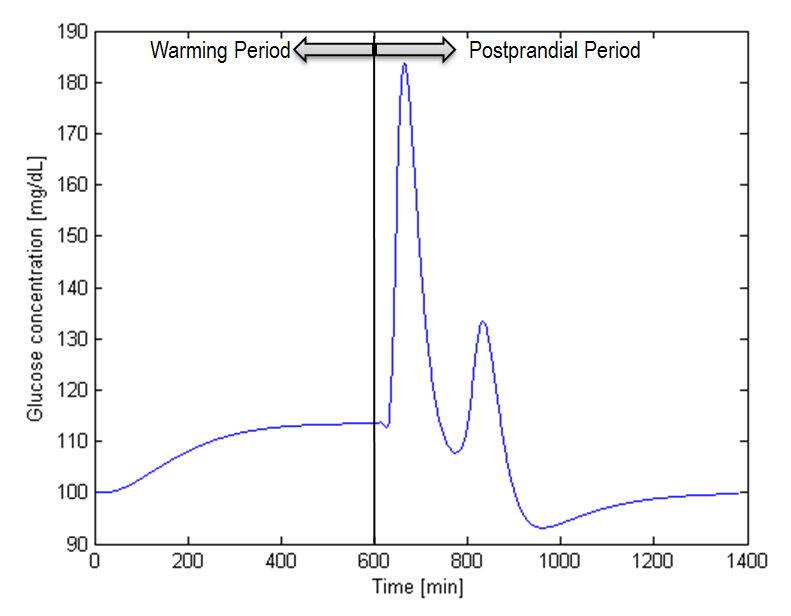
\epsfig{file=Figures/Bergmannobasal.png, width=0.8\textwidth}\caption{Bergman model simulation of a stop in the basal insulin infusion with nominal values of glucose effectiveness. Basal infusion is restored when the postprandial period begins.}
\label{fig:compare1}
\end{figure}

A small increase in glucose level can be seen as a consequence of the elimination of insulin infusion. Basal insulin removal causes a change in the settling point of the output variable, \textit{i.e.} glucose concentration. If basal insulin infusion stops in a model with smaller glucose effectiveness, the results are shown in Figure \ref{fig:compare2}.

\begin{figure}[hbtp]
\centering
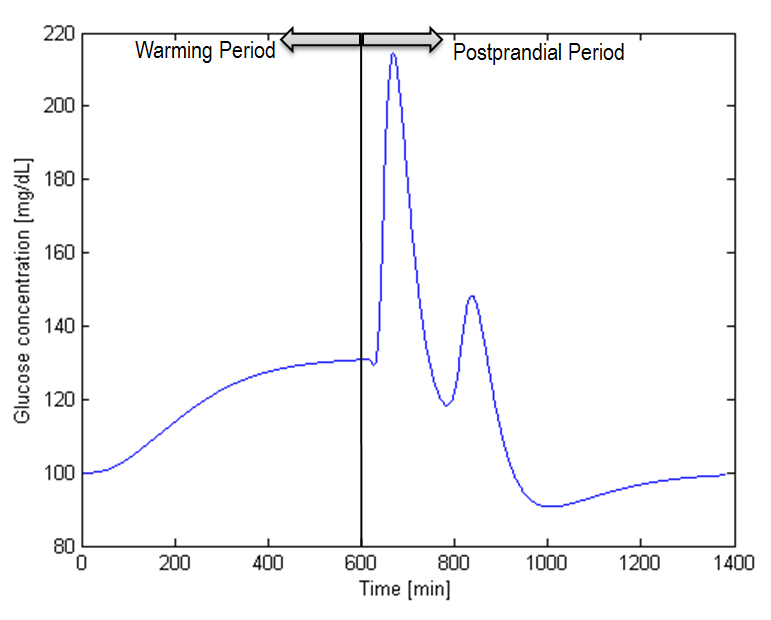
\epsfig{file=Figures/Bergmannobasal50percent.png, width=0.8\textwidth}\caption{Bergman model simulation of a stop in the basal insulin infusion with 50\% reduction in glucose effectiveness.}
\label{fig:compare2}
\end{figure}

The behavior observed in the ``warming'' period of Figures \ref{fig:compare1} and \ref{fig:compare2} is unrealistic. A diabetic patient whose insulin infusion is removed should become an unstable process, not just change its equilibrium point. Panunzi's model, in its equation (\eqref{eq:analysis2}) becomes a pure integrator if insulin is removed, making the system unstably increasing. Panunzi's model seems more suited to the physiology of glucose in diabetic patients in this case, but it also has its disadvantages. As it was said before, the Panunzi model represents the delay of insulin action in the equation of secretion, but that equation (\eqref{eq:Panunzi2}) is eliminated when simulating diabetic patients because of the absolute insulin deficiency in T1DM, so the delay effect is removed as well. If the delay is not reinstated somehow, the model simulates much faster dynamics when applying the bolus insulin in front of the simultaneous meal ingestion, making blood glucose to drop immediately after the injection, as can be seen in Figure \ref{fig:compare3}.

\begin{figure}[hbtp]
\centering
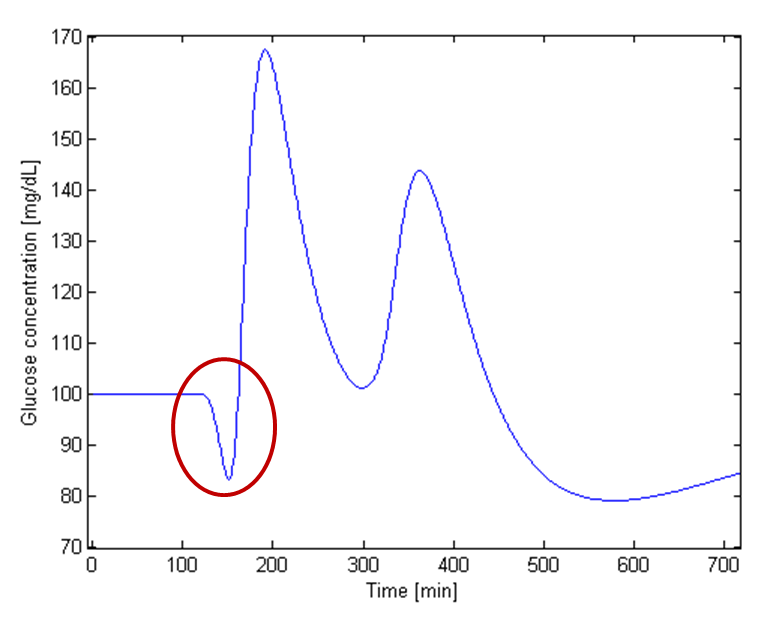
\epsfig{file=Figures/degaetano.png, width=0.8\textwidth}\caption{Panunzi model simulation of a postprandial period. Meal ingestion occurs at minute 120. Blood glucose drop after insulin bolus administration and before meal glucose appears into bloodstream is circled.}
\label{fig:compare3}
\end{figure}

This phenomenon is too pronounced and unrealistic. Even though insulin dynamics can, and often are, faster than gastrointestinal absorption, the effect on the displayed simulation is too abrupt and can yield to danger to the simulated patient. However, this effect can be easily avoided by adding a simple dynamic delay equation (\eqref{eq:analysis4}) to Panunzi's model, resulting in the next system of equations:
\begin{align}
  \dot{G}(t) &= -K_{xgl}X(t)G(t) +\frac{T_{gh}}{V_{g}} \label{eq:analysis3} \\
  \dot{X}(t) &= -k_{i}[X(t)-I(t)] \label{eq:analysis4}
\end{align}
With the addition of a new parameter to the model. This new parameter is not tuned and requires a nominal value to be set. This can be done simply by reviewing related literature. In \cite{helms2009insulin} Helms \& Kelley quantify the regular insulin action delay with a 30 minutes settling time. By looking at the new delay equation as a first order model, the time constant of the system can be calculated by assuming that the settling time is $3\times \tau$ (being $\tau$ the system's time constant), which reads a time constant of 10 minutes, and the parameter $k_{i}$ results to be equal to $0.1$ min$^{-1}$. The nominal parameter of this delay is dependent on the type of insulin being used, and it should be subject to deeper identification studies in the future. The response to a meal and a bolus in that case is shown in Figure \ref{fig:compare4}, where the dropping of glucose just after the bolus time is almost non present.

\begin{figure}[hbtp]
\centering
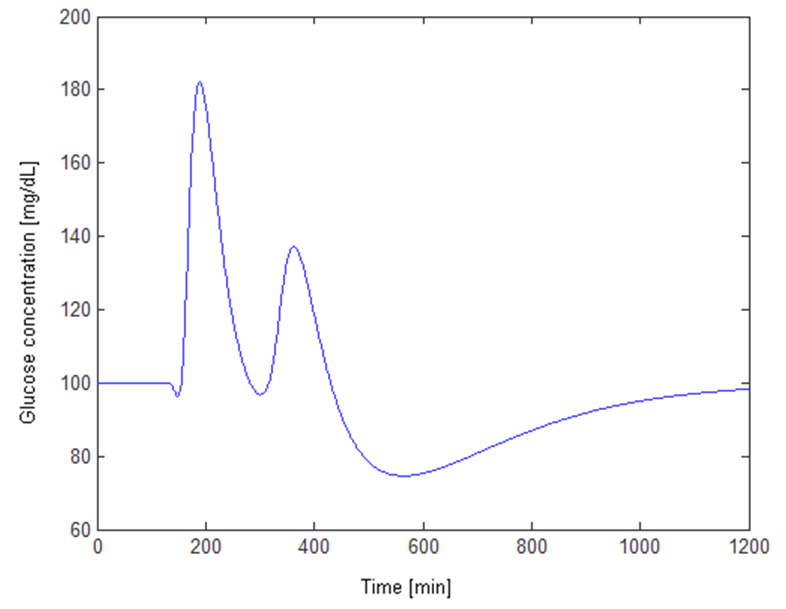
\epsfig{file=Figures/compare4.png, width=0.8\textwidth}\caption{Modified Panunzi model simulation of a postprandial period. Meal ingestion occurs at minute 120.}
\label{fig:compare4}
\end{figure}

The shown model is completely satisfactory for identification purposes and control. In order to check the model's reliability we look upon the work of 1994 by Torlone \textit{et al.} \cite{torlone1994}, where they showed a series of experiments in which insulin bolus is injected few minutes prior to an intravenous glucose infusion (infused in order to avoid hypoglycemia). This experiment shows clearly the effect and dynamics of insulin, and how it makes glucose to decrease in a similar way to an impulse response. From the work done by Torlone \textit{et al.} it can be extracted that there is no significant change in blood glucose until approximately 15 minutes after bolus injection, and then glucose drops steadily for 30 minutes until approximately 70 mg/dL (approximately 3 $mmol/l$). A very similar set-up was used for simulating the modification of Panunzi's model including insulin delay; an insulin bolus was applied and the effect on the blood glucose measured, as displayed in Figure \ref{fig:compare5}, but no intravenous glucose infusion was simulated.
%In Figure \ref{fig:perugia} insulin action is applied separately from any other action for almost one hour before the glucose infusion starts.

%\begin{figure}[hbtp]
%\centering
%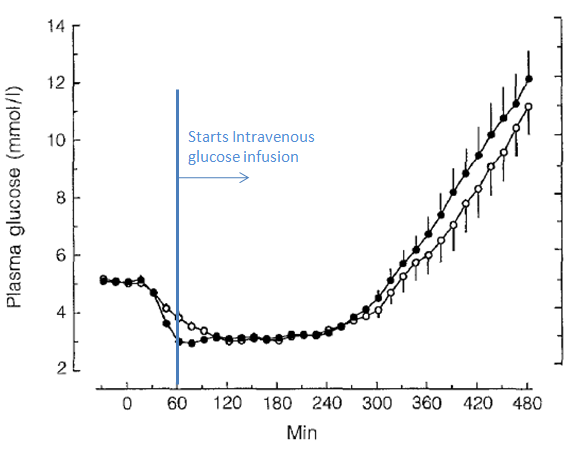
\epsfig{file=Figures/perugia.png, width=0.8\textwidth}\caption{Insulin impulse response of glucose after bolus and counteraction with intravenous glucose infusion \cite{torlone1994}. Black %dots represent the blood glucose measurements for monomeric insulin analog, and the white dots for human insulin.}
%\label{fig:perugia}
%\end{figure}

\begin{figure}[hbtp]
\centering
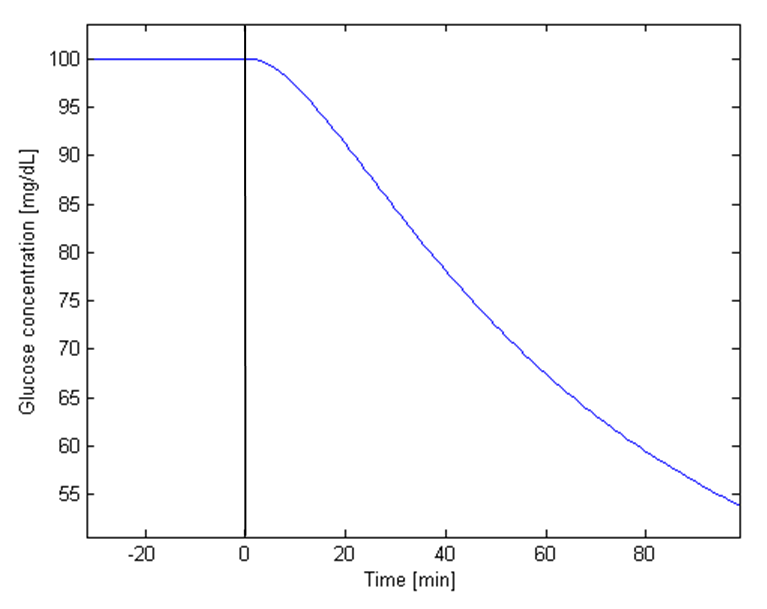
\epsfig{file=Figures/modifiedpanunzisimulation.png, width=0.8\textwidth}\caption{Variation of blood glucose (mg/dL) in Panunzi's model simulating a drop of glucose after insulin injection. Insulin is given at time $0$.}
\label{fig:compare5}
\end{figure}

In simulation, the response is exactly as expected: no significant change in blood glucose in the first minutes, and in the next half hour, glucose level drops to almost 70 mg/dL. This new dynamics make the new model much more reliable than Bergman or Panunzi's models in the referent to insulin simulation, and also proves valid the artificial delay added to the insulin action.

Another simple feature has also been included in the modified Panunzi model. Endogenous hepatic glucose production is one of the parameters of the model, $T_{gh}$, and it is considered constant. This parameter is actually variable, because endogenous hepatic production is suppressed by insulin. A simple variation of the model has been introduced, considering the $T_{gh}$ parameter to be reduced when plasma insulin surpassed a defined threshold, and defined as a piecewise function as follows:

\begin{equation} 
  T_{gh}=\left\{ \begin{array}{cc} 
  T_{gh0} & \mbox{ if } I(t) < T_{gh thr} \mbox{ }mIU/l\\ 
  K_{gh}\cdot T_{gh0} & \mbox{ otherwise } \\	
  \end{array} \right.
\label{eq:tegehache}
\end{equation}

where $T_{gh thr}$ is the above mentioned insulin threshold, $T_{gh0}$ is the basal endogenous production and $K_{gh}$ is the glucose production factor. 

With the described changes applied to Panunzi's model, a very useful yet simple model was developed and can be used for identification and identifiability studies in the following thesis. This resulting model will be mentioned in this thesis as ``Modified Panunzi Model'' 

